\documentclass{standalone}
\usepackage{tikz}
\usetikzlibrary{fit, positioning, arrows.meta, calc, backgrounds}
\usepackage{xcolor}

\definecolor{apibg}{RGB}{245,245,235}
\definecolor{uibg}{RGB}{220,235,250}

\begin{document}

% Modules are placed on an explicit grid so that every dependency runs
% downwards:  columns x = 0, 5, 10   rows y = 0, -1.45, -2.9, -4.35.
% The empty grid cells are deliberate -- they hold the group labels and the
% routed edges (treeflow.tree -> distributions.tree, tree.io -> cli).
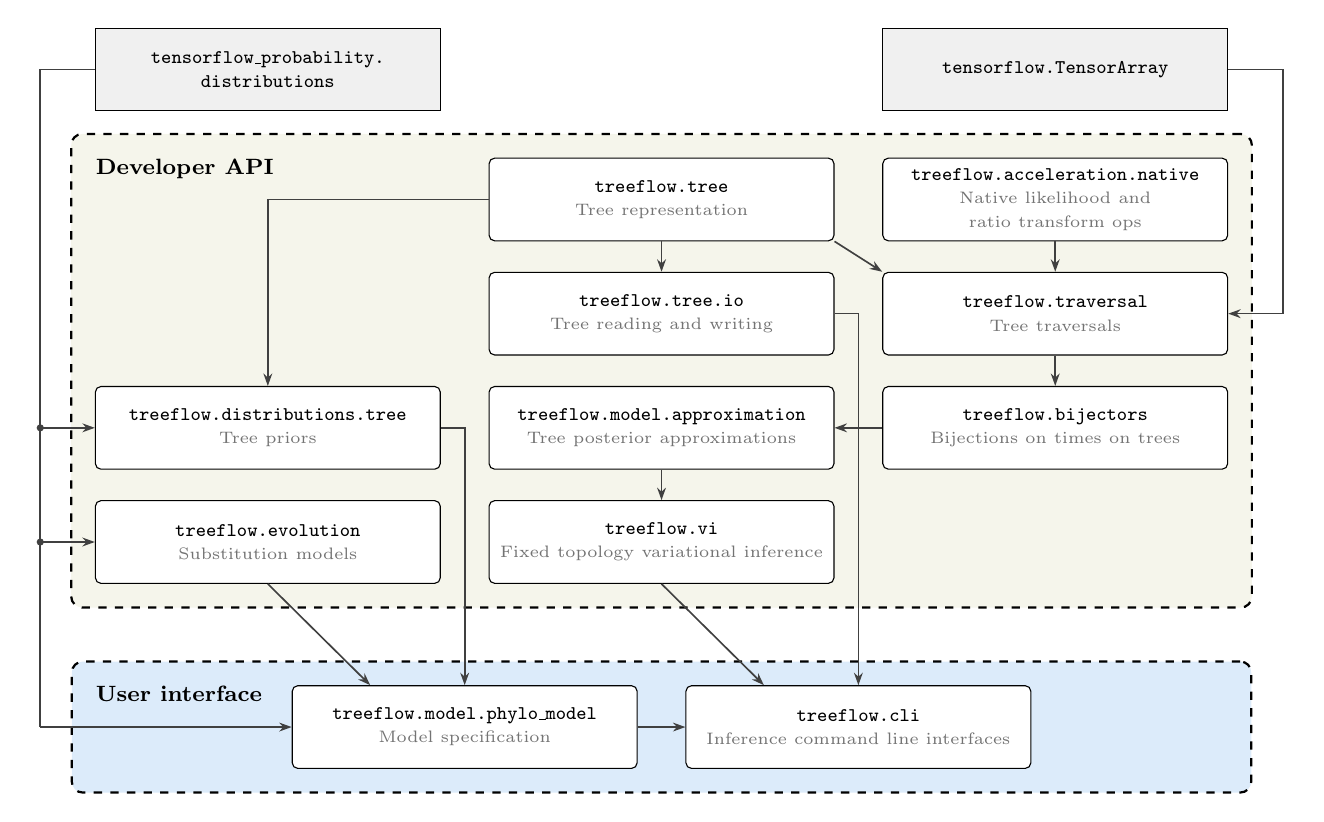
\begin{tikzpicture}[
        x=1cm, y=1cm,
        box/.style={draw, rounded corners=2pt, fill=white, align=center,
                    text width=4.1cm, inner xsep=0.14cm, inner ysep=0.12cm,
                    minimum height=1.05cm, font=\fontsize{7}{8.4}\selectfont},
        depbox/.style={box, rounded corners=0pt, fill=black!6},
        apifitbox/.style={draw, thick, dashed, rounded corners=4pt,
                          inner sep=0.3cm, fill=apibg},
        uifitbox/.style={draw, thick, dashed, rounded corners=4pt,
                         inner sep=0.3cm, fill=uibg},
        grouplabel/.style={font=\bfseries\fontsize{8}{9.6}\selectfont,
                           inner sep=0pt, anchor=north west},
        arrow/.style={-{Stealth[length=4.5pt,width=3.2pt]}, semithick, black!75},
        bus/.style={semithick, black!75},
        junction/.style={circle, fill=black!75, inner sep=0pt, minimum size=2.6pt},
    ]

    % keep line spacing inside nodes independent of the host document
    % (the manuscript is set double-spaced around the figure)
    \renewcommand{\baselinestretch}{1}\selectfont

    \def\dsc{\fontsize{6}{7}\selectfont\color{black!55}}

    % ---------- Developer API modules ------------------------------------
    \node[box] (tree)          at ( 5.0,  0.0) {\texttt{treeflow.tree}\\{\dsc Tree representation}};
    \node[box] (native)        at (10.0,  0.0) {\texttt{treeflow.acceleration.native}\\{\dsc Native likelihood and ratio transform ops}};

    \node[box] (io)            at ( 5.0, -1.45) {\texttt{treeflow.tree.io}\\{\dsc Tree reading and writing}};
    \node[box] (traversal)     at (10.0, -1.45) {\texttt{treeflow.traversal}\\{\dsc Tree traversals}};

    \node[box] (priors)        at ( 0.0, -2.9) {\texttt{treeflow.distributions.tree}\\{\dsc Tree priors}};
    \node[box] (approximation) at ( 5.0, -2.9) {\texttt{treeflow.model.approximation}\\{\dsc Tree posterior approximations}};
    \node[box] (bijectors)     at (10.0, -2.9) {\texttt{treeflow.bijectors}\\{\dsc Bijections on times on trees}};

    \node[box] (evolution)     at ( 0.0, -4.35) {\texttt{treeflow.evolution}\\{\dsc Substitution models}};
    \node[box] (vi)            at ( 5.0, -4.35) {\texttt{treeflow.vi}\\{\dsc Fixed topology variational inference}};

    \node[grouplabel] (apilabel) at (-2.19, 0.525) {Developer API};

    \begin{pgfonlayer}{background}
        \node[apifitbox, fit=(apilabel)(tree)(native)(io)(traversal)
                             (priors)(approximation)(bijectors)(evolution)(vi)]
              (developerapi) {};
    \end{pgfonlayer}

    % ---------- User interface -------------------------------------------
    \node[box] (phylomodel) at (2.5, -6.7) {\texttt{treeflow.model.phylo\_model}\\{\dsc Model specification}};
    \node[box] (cli)        at (7.5, -6.7) {\texttt{treeflow.cli}\\{\dsc Inference command line interfaces}};

    \node[grouplabel] (uilabel) at (-2.19, -6.175) {User interface};
    \coordinate (uipad) at (12.19, -6.7);

    \begin{pgfonlayer}{background}
        \node[uifitbox, fit=(uilabel)(phylomodel)(cli)(uipad)] (userinterface) {};
    \end{pgfonlayer}

    % ---------- External dependencies ------------------------------------
    \node[depbox] (tfp)         at ( 0.0, 1.65) {\texttt{tensorflow\_probability.}\\\texttt{distributions}};
    \node[depbox] (tensorarray) at (10.0, 1.65) {\texttt{tensorflow.TensorArray}};

    % ---------- Dependencies inside the developer API ---------------------
    \draw[arrow] (tree) -- (io);
    \draw[arrow] (tree.south east) -- (traversal.north west);
    \draw[arrow] (tree.west) -| (priors.north);
    \draw[arrow] (native) -- (traversal);
    \draw[arrow] (traversal) -- (bijectors);
    \draw[arrow] (bijectors.west) -- (approximation.east);
    \draw[arrow] (approximation) -- (vi);

    % ---------- Developer API -> user interface ---------------------------
    \draw[arrow] (priors.east) -- (2.5,-2.9) -- (phylomodel.north);
    \draw[arrow] (evolution.south) -- ([xshift=-1.2cm]phylomodel.north);
    \draw[arrow] (io.east) -- (7.5,-1.45) -- (cli.north);
    \draw[arrow] (vi.south) -- ([xshift=-1.2cm]cli.north);
    \draw[arrow] (phylomodel) -- (cli);

    % ---------- External dependency buses ---------------------------------
    \draw[bus]   (tfp.west) -- (-2.89,1.65) -- (-2.89,-6.7);
    \draw[arrow] (-2.89,-2.9) -- (priors.west);
    \draw[arrow] (-2.89,-4.35) -- (evolution.west);
    \draw[arrow] (-2.89,-6.7) -- (phylomodel.west);
    \node[junction] at (-2.89,-2.9) {};
    \node[junction] at (-2.89,-4.35) {};

    \draw[arrow] (tensorarray.east) -- (12.89,1.65) -- (12.89,-1.45) -- (traversal.east);

    % small margin around the dependency buses
    \path (-3.05,0) (13.05,0);

\end{tikzpicture}

\end{document}
